\documentclass[a4paper,12pt]{article}

% Pour le bon support de la langue française : 
\usepackage[utf8]{inputenc}
\usepackage[T1]{fontenc}
\usepackage[english, francais]{babel}

\usepackage{lipsum} % \lipsum créera un texte test
\usepackage[margin=2.4cm]{geometry} %pour des marges

\usepackage{framed} % des contours
\usepackage[framed]{ntheorem} % un théoreme



\usepackage[all]{xy}
%
\usepackage{listings}

\usepackage{hyperref}

\hypersetup{
    bookmarks=true,         % show bookmarks bar?
    unicode=false,          % non-Latin characters in Acrobat’s bookmarks
    pdftoolbar=true,        % show Acrobat’s toolbar?
    pdfmenubar=true,        % show Acrobat’s menu?
    pdffitwindow=false,     % window fit to page when opened
    pdfstartview={FitH},    % fits the width of the page to the window
    pdfnewwindow=true,      % links in new PDF window
    colorlinks=true,       % false: boxed links; true: colored links
    linkcolor=blue,          % color of internal links (change box color with linkbordercolor)
    citecolor=magenta,        % color of links to bibliography
    filecolor=magenta,      % color of file links
    urlcolor=cyan           % color of external links
}

\let\urlorig\url
\renewcommand{\url}[1]{%
   \begin{otherlanguage}{english}\urlorig{#1}\end{otherlanguage}%
}


% Bibliographie dans la Table des matières
\usepackage[nottoc, notlof, notlot]{tocbibind}



\usepackage{tikz}               % Tracer des graphes
\tikzset{every picture/.style={execute at begin picture={
\shorthandoff{:;!?};}
}}


\usepackage{thumbpdf}           % Fichier pdf généré 
                                % contien une              
                                % miniature de chaque slide 

 \usepackage{dsfont}
\usepackage{lastpage}           % Avoir total de pages dans le footer.
\usepackage{graphicx}           % Pour les images et figures
\usepackage{wrapfig}            % Pour détourer les figures
\usepackage{fancybox}           % De chouettes encadrements
\usepackage{lettrine}           % Pour de beaux paragraphes
\usepackage{setspace}           % Pour changer l'interligne
\usepackage{eurosym}            % Pour le signe \euro
\usepackage{xcolor}             % Pour mettre d la couleur
\usepackage{colortbl}           % Couleur dans tableaux
\usepackage{tabularx}           % pour des tableaux à taille de la page
\usepackage{longtable}          % Pour les grands tableaux
\usepackage[tight]{shorttoc}    % Pour faire un sommaire à la française.
\newcommand{\sommaire}{\shorttoc{Sommaire}{1}}
\usepackage{array}              % De beaux tableaux
\usepackage{multirow}           % Tableaux sur plusieurs lignes
                                % \multirow{nlignes}{largeur ou *}{contenu}
\usepackage{amsmath}            % Un peu de maths
\usepackage{amssymb}            % Encore des maths
\usepackage{mathtools}
\usepackage{empheq}             % Pour encadrer les équations


\usepackage{stmaryrd}			% pour les crochets d'intervalles entiers 


\usepackage{pgfpages}           % Pour avoir 2 pages sur A4 paysage
\usepackage{datetime}           % Jouer facilement avec les dates
% Pour la physique : 
\usepackage{numprint}           % Pour faire des groupes de 3 nombres
\usepackage[squaren,Gray,cdot]{SIunits}

\usepackage{pgf}
\usetikzlibrary{arrows}

\usepackage{nameref} %pour les entetes 
\makeatletter
\newcommand*{\currentname}{\@currentlabelname}
\makeatother

\definecolor{vert}{rgb}{0,0.6,0}
\definecolor{mauve}{rgb}{0.58,0,0.82}

\lstset{ %
  backgroundcolor=\color{white},   % choose the background color
  breaklines=true,                 % automatic line breaking only at whitespace
  captionpos=b,                    % sets the caption-position to bottom
  commentstyle=\color{vert},    % comment style
  escapeinside={\%*}{*)},          % if you want to add LaTeX within your code
  keywordstyle=\color{blue},       % keyword style
  stringstyle=\color{mauve},     % string literal style
  basicstyle=\small\ttfamily,%
  frame=single,
  mathescape=true,
  %extendedchars=true,
 literate=%
         {é}{{\'e}}1
         {É}{{\'E}}1
         {à}{{\`a}}1
         {ê}{{\^e}}1
         {è}{{\`e}}1
}

%%%
% Commandes
\newcommand{\ndiv}{\nmid} %x\ndiv y <==> x ne divise pas y
\newcommand{\modulo}[3]{#1\equiv #2 \;[#3]}
\newcommand{\nmodulo}[3]{#1\not\equiv #2 \;[#3]}


% Ajout d'une image avec label
\newcommand{\image}[3]{
% \image{fichier}{label}{description}
\begin{center}
% Nécessite le package float
\begin{figure}[H]
\includegraphics[width=0.9\textwidth]{#1}
\caption{\label{#2}{#3}}
\end{figure}
\end{center}
}

% Ajout d'une image largeur page avec label
\newcommand{\imagebig}[3]{
% \imagebig{fichier}{label}{description}
\begin{center}
% Nécessite le package float
\begin{figure}[H]
\includegraphics[width=\textwidth]{#1}
\caption{\label{#2}{#3}}
\end{figure}
\end{center}
}

% Une image qui prend toute la page
\newcommand{\imagefull}[1]{
    \newgeometry{margin=0cm}
\begin{center}
\begin{figure}[H]
\includegraphics[width=0.96\paperwidth]{#1}
\end{figure}
\end{center}
\restoregeometry
\nopagebreak
}

% Un encadré grisé
\newcommand{\encadregris}[1]{
\begin{center}
\colorbox{gray!20}{
\begin{minipage}{0.95\textwidth}
{#1}
\end{minipage}
}
\end{center}
}

% Un mot grisé
\newcommand{\motgris}[1]{
\colorbox{gray!20}{{#1}}
}

% Un encadré
\newcommand{\encadre}[1]{
\begin{center}
\fbox{
\begin{minipage}{\textwidth}
{#1}
\end{minipage}
}
\end{center}
}

%Une boite coloré
\newenvironment{colbox}[1]
{\def\FrameCommand{\colorbox{#1}}%
   \MakeFramed{\advance\hsize-\width \FrameRestore}}
{\endMakeFramed}

\colorlet{shadecolor}{blue!8}

%%%%%%%%%% Des Maths %%%%%%%%%%%%%%

\newcommand{\RR}{\ensuremath{\mathbb{R}}}
\newcommand{\CC}{\ensuremath{\mathbb{C}}}
\newcommand{\ZZ}{\ensuremath{\mathbb{Z}}}
\newcommand{\QQ}{\ensuremath{\mathbb{Q}}}
\newcommand{\NN}{\ensuremath{\mathbb{N}}}
\newcommand{\PP}{\ensuremath{\mathbb{P}}}
\newcommand{\KK}{\ensuremath{\mathbb{K}}}
\newcommand{\EE}{\ensuremath{\mathbb{E}}}
\renewcommand{\SS}{\ensuremath{\mathbb{S}}}
\newcommand{\TT}{\ensuremath{\mathbb{T}}}

\newcounter{theo}[section] % créer un nouveau compteur
\renewcommand\thetheo{\thesection.\arabic{theo}}
\newcounter{prop}[section]
\renewcommand\theprop{\thesection.\arabic{prop}}

\newenvironment{theoreme}[1]
{\refstepcounter{theo}\begin{shaded}\textbf{Théorème \thetheo~ : } \textit{#1}\vspace{0.3em}
\hrule
\medbreak}
{\end{shaded}}


\newenvironment{propriete}
{\begin{shaded}\textbf{Propriété : }\\ }
{\end{shaded}}

\newenvironment{proposition}
{\refstepcounter{prop}\begin{shaded}\textbf{Proposition \theprop~ : }\\ }
{\end{shaded}}

\newenvironment{corollaire}
{\begin{shaded}\textbf{Corollaire : }\\ }
{\end{shaded}}


\newenvironment{lemme}
{\begin{shaded}\textbf{Lemme : }\\ }
{\end{shaded}}


\newenvironment{definition}[1]
{\stepcounter{theo}\begin{shaded}\textbf{Définition \thetheo~ : } \textit{#1}\vspace{0.3em}
\hrule
\medbreak}
{\end{shaded}}

\newlength{\mylength}
\setlength{\mylength}{\linewidth}
\addtolength{\mylength}{-2\fboxsep}
\addtolength{\mylength}{-2\fboxrule}

\newenvironment{boxeq}{\setlength{\fboxsep}{15pt}
\setlength{\mylength}{\linewidth}%
\addtolength{\mylength}{-2\fboxsep}%
\addtolength{\mylength}{-2\fboxrule}%
\Sbox
\minipage{\mylength}%
\setlength{\abovedisplayskip}{0pt}%
\setlength{\belowdisplayskip}{0pt}%
\equation}%
{\endequation\endminipage\endSbox
\[\fbox{\TheSbox}\]}


\newcounter{exos}
\newcommand{\exo}[1]{\stepcounter{exos}\Ovalbox{Exercice \theexos} \textbf{#1}}
\newcommand{\attention}[1]{\textcolor{red!90}{\textbf{Attention :} #1 }}
\newcommand{\remarque}[1]{\textcolor{blue!90}{\textbf{Remarque :} #1 }}
\newcommand{\exemple}[1]{\textcolor{magenta!80}{\textbf{Exemple :} #1 }}
\newcommand{\remarques}[1]{\textcolor{blue!90}{\textbf{Remarques :} #1 }}


\newenvironment{preuve}
{\begin{leftbar}\textbf{Preuve :} \\ }
{\hfill\ensuremath{\Box}\end{leftbar}\medbreak}




% flèche
\newcommand{\ra}[0]{
    $\rightarrow$
}




% Image détourée
% \wrapimg{align}{width}{img}
\newcommand{\wrapimg}[3]{
\begin{wrapfigure}{#1}{#2}
\includegraphics[width={#2}]{#3}
\end{wrapfigure}
}

\newcommand{\hdr}[0]{
    \hdashrule{1cm}{1pt}{1pt}
}

\newcommand*{\etoile}
{
\begin{center}
*\par
*\hspace*{3ex}*
\end{center}
}


% listes avec puces carrées
\newcommand{\carlst}[1]{
    \begin{itemize}
    \renewcommand\labelitemi{\petitcarre}
    {#1}
    \end{itemize}
}





\usepackage{tikz,tkz-tab}
\csname @addtoreset\endcsname{section}{part} 

\newcommand{\fonction}[5]{\ensuremath{\begin{array}[t]{l|ccl}
#1: & #2 & \longrightarrow & #3 \\
    & #4 & \longmapsto & #5 \end{array}}}






% MISE EN FORME DU TITRE
\makeatletter
\renewcommand{\maketitle}{

\begin{minipage}[l]{.8\linewidth}

\includegraphics[width=120px]{img/logo.png} %logo insa
\end{minipage} \hfill
\begin{minipage}[r]{.46\linewidth}

\includegraphics[width=100px]{img/logo_cologne.png}
\end{minipage}


\vspace{3cm}
\begin{center}
\boxput*(0,1){\colorbox{white}{Internship Repport}}{
\setlength{\fboxsep}{10pt}
\framebox[\textwidth]{
\begin{minipage}{8cm}
\center
\Large
\@title
\end{minipage}
}}
\end{center}

\vspace{1cm}
\begin{center}
Universität zu Köln\\
INSA de Rouen Normandie - \dateDoc
\end{center}


\vspace{1cm}
\begin{figure}[!h]
\centering
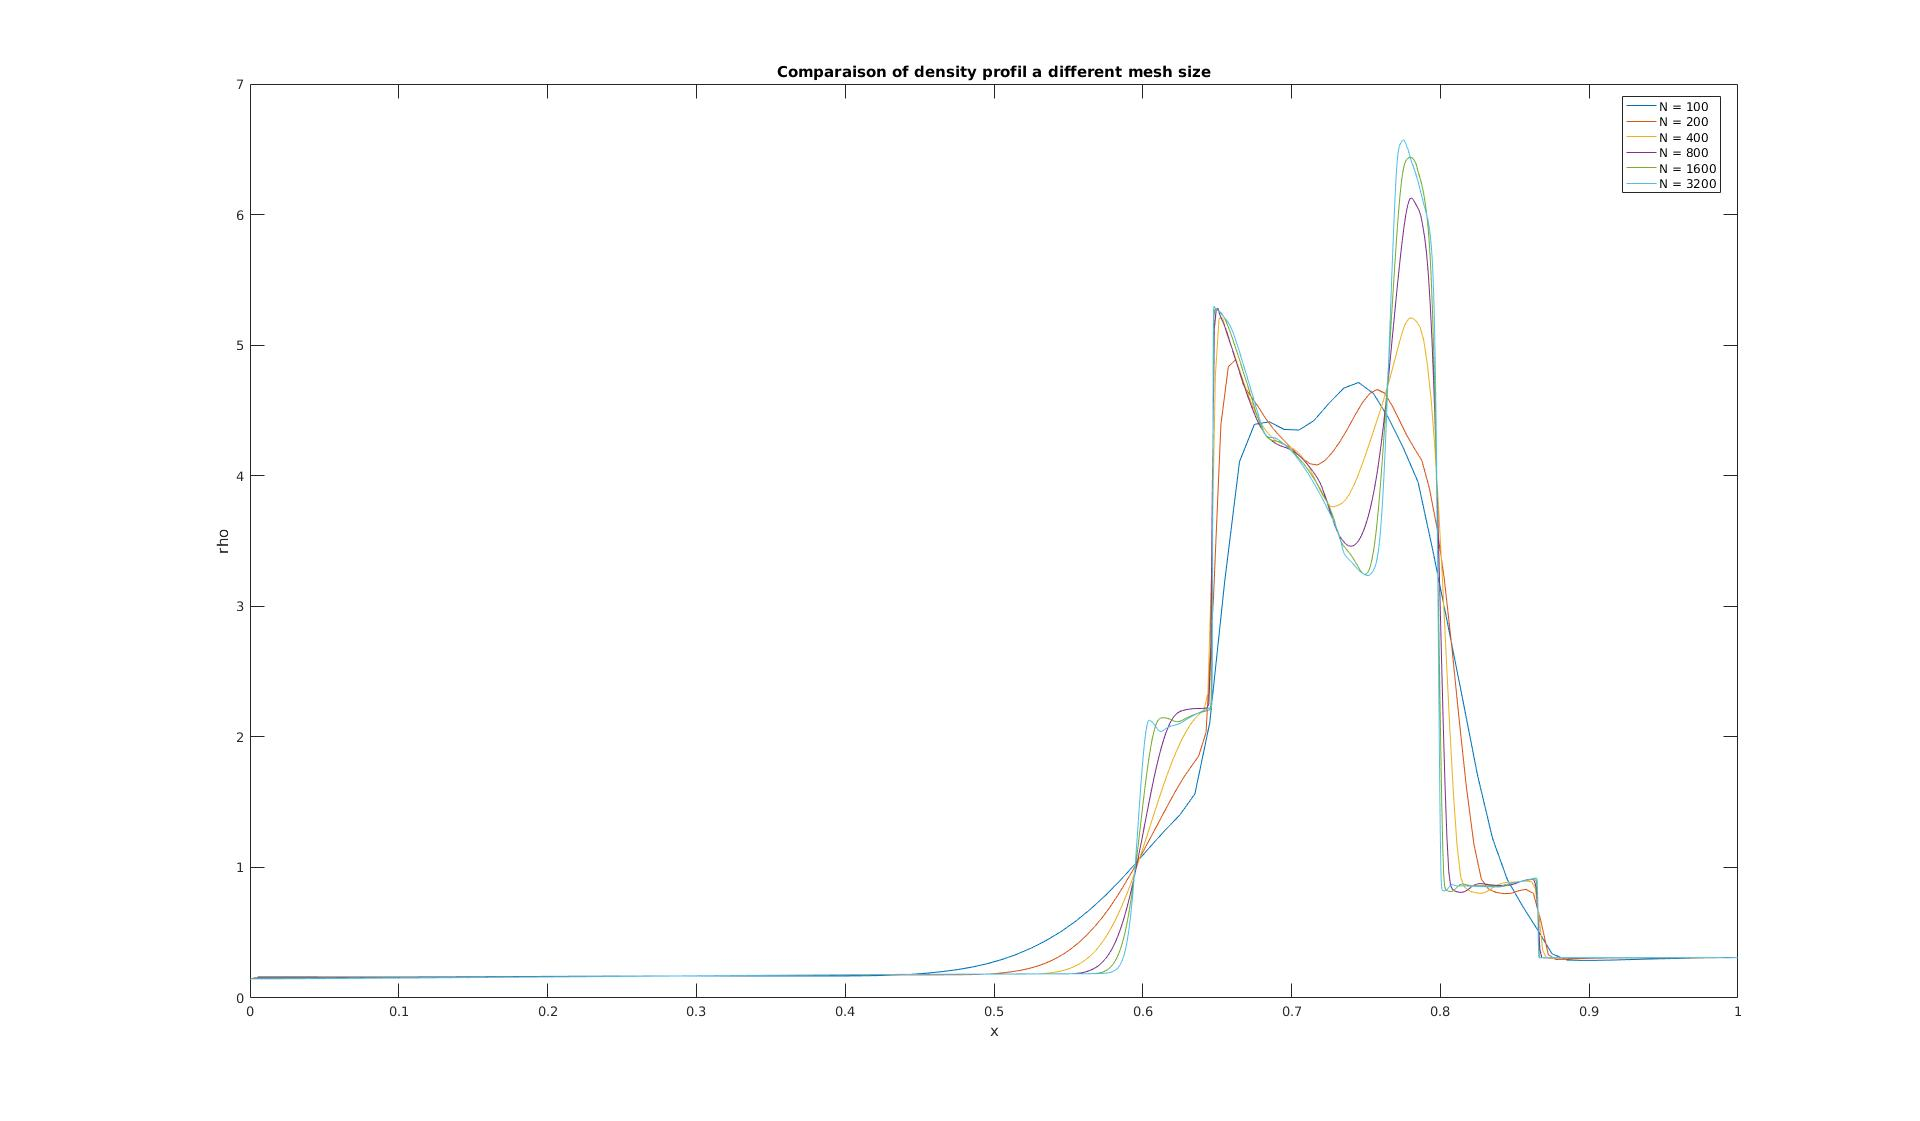
\includegraphics[width=400px]{img/main.jpg} %logo du document
\end{figure}


\vspace{1cm}
\begin{minipage}[l]{0.4\textwidth}
\large
\emph{Author :}\\
\@author\\
\end{minipage}
\hfill
\begin{minipage}[r]{0.4\textwidth}
\large
\flushright
\emph{Referent :} \\
Gregor \textsc{Gassner}\\ % Supervisor's Name
XXXX \textsc{XXXX}
\end{minipage}
\newpage
}
\makeatother
%%%


%\begin{center}
%\vspace{2ex}
%{\huge \textsc{\@title}}
%\vspace{1ex}
%\\
%\linia\\
%\@author \hfill \@date
%\vspace{4ex}
%\end{center}

%\begin{tcolorbox}[enhanced,attach boxed title to top center={yshift=-3mm,yshifttext=-1mm},
 % colback=blue!5!white,colframe=blue!75!black,colbacktitle=red!80!black,
  %title=My title,fonttitle=\bfseries,
  %boxed title style={size=small,colframe=red!50!black} ]
  %This box uses a \textit{boxed title}. The box of the title can
  %be formatted independently from the main box.
%\end{tcolorbox}









\setlength{\parindent}{0pt}
\newcommand\titre{Non regular Nodes method for Euler Gas Equation}
\newcommand\auteur{Timothée \textsc{Schmoderer}}
\newcommand\dateDoc{2017}
\newcommand\chapitre{Chapitre 2}
\newcommand\cours{Internship Repport}
\usepackage{enumitem}
\everymath{\displaystyle}

\title{\titre }
\author{\auteur}
\date{\dateDoc}

\usepackage{fancyhdr,lastpage}
\pagestyle{fancy}

\lhead{\cours}
\chead{}
\rhead{\currentname}
\lfoot{\titre}
\cfoot{}
\rfoot{Page \thepage\ /\ \pageref*{LastPage}}  


\lstset{
language=Matlab,
}

\hypersetup {
 pdftitle={\titre},    % title
    pdfauthor={\auteur},     % author
    pdfsubject={\cours},   % subject of the document
    pdfkeywords={flot optique, Horn, schunck, image, projet}, % list of keywords
}


\renewcommand{\lstlistingname}{Code}% Listing -> Code
\renewcommand{\lstlistlistingname}{List of \lstlistingname s}% List of Listings -> List of codes



\begin{document}
\thispagestyle{empty}
\maketitle
\tableofcontents
\newpage

\section{Introduction}


\newpage

\section{Euler Gas Equation}
Let's begin with a brief introduction about the euler gas equations (\cite{wiki:EulerGasEquation}). These equations descibe fluid behaviour when we could consider that there is no viscosity. That is to say especially for gas. For a one dimensionnal system, the equations are written as follow : 

\begin{boxeq}
\frac{\partial}{\partial t} 
\begin{pmatrix}
\rho\\
\rho u\\
E
\end{pmatrix}  +
\frac{\partial}{\partial x}
\begin{pmatrix}
\rho u \\
P + \rho u^2\\
u(E+P)
\end{pmatrix}
=0
\label{eq:EulerGasEquation}
\end{boxeq}

\paragraph{Convention :} This system illustrates a convention we will systematically make. The partial derivative are intends to act on each components of the vectors. \\
\newline
Where : 
\begin{enumerate}
\item $\rho$ stands for the density is strictly positive. 
\item $P$ stands for the presure and is also strictly positive. 
\item $E$ is the internal energy 
\item $u$ is the gas velocity which could be either positive (if gas is moving toward increasing value in space) or negative.
\end{enumerate}

All this variable depends of time and space. The system (\ref{eq:EulerGasEquation}) is close by a fourth equation, an equation of state which bound pressure, density and energy : 
\begin{boxeq}
E = \frac{P}{\gamma -1} -\frac{\rho u^2}{2}
\label{eq:equationOfState}
\end{boxeq}
Where $\gamma$ is some gas constant coming from adiabatic. It will be taken equal to : $1.4$. 

We will also need to compute the speed of sound in the gas, this is givern by : 
$$
c = \sqrt{\frac{\gamma P}{\rho}}
$$
In general there is no analytic solution of this system, which will lead us to knew technique of convergence rate analysis. \\
The system \ref{eq:EulerGasEquation} describe non linear hyberpolics partial differential equations. The difficulties is that even is the initial conditiosn are smooth, the solution could present discontinuities, or in a more physical vocabulary, chock waves. This is a major problem to construct numerical method to capture them. \\
\newline
To put the system \ref{eq:EulerGasEquation} is a more compact way, let $U=\begin{pmatrix}
\rho\\
\rho u\\
E
\end{pmatrix}$ be the state vector and $f(U)=\begin{pmatrix}
\rho u \\
P + \rho u^2\\
u(E+P)
\end{pmatrix}$ be the flux vector such as \ref{eq:EulerGasEquation} rewrite as : 
$$
\frac{\partial U}{\partial t}+ \frac{\partial f(U)}{\partial x} = 0
$$


\subsection{The problem}
In this etud, the domain is taken to be : $\Omega=[0,1]$ and the time in $[0,0.1]$
The problem is closed with proper boundary and initial conditions : 
\begin{boxeq}
\begin{split}
u(0)=u(1)&=0\\
\frac{\partial \rho}{\partial x} \bigg\rvert_{x=0,1} &=0\\
\frac{\partial P}{\partial x} \bigg\rvert_{x=0,1} &=0\\
u(x,0) &= 0 \quad \forall x\in \Omega\\
\rho(x,0) &= 1 \quad \forall x\in \Omega\\
P(x,0)&= \left\{ \begin{array}{ccc}
1000 & \text{if  } 0<x<0.1\\
0.01 & \text{if  } 0.1<x<0.9\\
100 & \text{if  } 0.9<x<1\\
\end{array} \right.
\end{split}
\label{eq:initialCondition}
\end{boxeq}

Which we can interpret as solid wall conditions on both extremities of the tubes. 

\subsection{Expecting results}
The initial condition suggests that at $t=0$ there is some kind of valves at $x= 0.1$ and $x=0.9$ that are oppened. After we can easy imagine that due to pressure the gas "want" to uniform his energy, so the left side will be moving to the right, the right side to the left. 
But what happend when this two wave coliddes ?

In fact due to the hyperbolic characteristics of the system \ref{eq:EulerGasEquation} we can expect chock waves. The numerical difficulties is to capture them. 

\section{Numerical scheme}
\subsection{General method for hyberbolic system}
\subsubsection{Cells and Nodes}
Choose a integer $N$ (obviously not null, we won't go far), and let divide $\Omega$ into $N$ grid "cells" (Figure \ref{fig:OmegaCells}), and let $x_i$ be the cell-centers. 
\begin{figure}[!h]
\centering
\definecolor{xdxdff}{rgb}{0.49,0.49,1}
\definecolor{ffqqqq}{rgb}{1,0,0}
\definecolor{cqcqcq}{rgb}{0.75,0.75,0.75}
\begin{tikzpicture}[line cap=round,line join=round,>=triangle 45,x=15.0cm,y=15.0cm]
\draw [color=cqcqcq,dash pattern=on 1pt off 1pt, xstep=0.75cm,ystep=0.75cm] (-0.03,-0.08) grid (1.03,0.07);
\clip(-0.03,-0.08) rectangle (1.03,0.07);
\draw (0,0)-- (1,0);
\draw (0,0.05)-- (0,-0.05);
\draw (0.1,0.05)-- (0.1,-0.05);
\draw (0.2,0.05)-- (0.2,-0.05);
\draw (0.3,0.05)-- (0.3,-0.05);
\draw (0.4,0.05)-- (0.4,-0.05);
\draw (0.5,0.05)-- (0.5,-0.05);
\draw (0.6,0.05)-- (0.6,-0.05);
\draw (0.7,0.05)-- (0.7,-0.05);
\draw (0.8,0.05)-- (0.8,-0.05);
\draw (0.9,0.05)-- (0.9,-0.05);
\draw (1,0.05)-- (1,-0.05);
\draw (-0.02,0.01) node[anchor=north west] {$ 0 $};
\draw (1,0.01) node[anchor=north west] {$ 1 $};
\draw (0.01,0.08) node[anchor=north west] {$ \text{cell } 1 $};
\draw (0.11,0.08) node[anchor=north west] {$ \text{cell } 2 $};
\draw (0.51,0.08) node[anchor=north west] {$ \text{cell } j $};
\draw (0.91,0.08) node[anchor=north west] {$ \text{cell } N $};
\draw (-0.01,-0.045) node[anchor=north west] {$ x_{1/2} $};
\draw (0.08,-0.045) node[anchor=north west] {$ x_{3/2} $};
\draw (0.18,-0.045) node[anchor=north west] {$ x_{5/2} $};
\draw (0.48,-0.045) node[anchor=north west] {$ x_{j-1/2} $};
\draw (0.58,-0.045) node[anchor=north west] {$ x_{j+1/2} $};
\draw (0.04,0) node[anchor=north west] {$ x_1 $};
\draw (0.14,0) node[anchor=north west] {$ x_2 $};
\draw (0.54,0) node[anchor=north west] {$ x_j $};
\begin{scriptsize}
\fill [color=ffqqqq] (0,0) circle (1.5pt);
\fill [color=ffqqqq] (1,0) circle (1.5pt);
\fill [color=xdxdff] (0.05,0) circle (1.5pt);
\fill [color=xdxdff] (0.15,0) circle (1.5pt);
\fill [color=xdxdff] (0.25,0) circle (1.5pt);
\fill [color=xdxdff] (0.35,0) circle (1.5pt);
\fill [color=xdxdff] (0.45,0) circle (1.5pt);
\fill [color=xdxdff] (0.55,0) circle (1.5pt);
\fill [color=xdxdff] (0.65,0) circle (1.5pt);
\fill [color=xdxdff] (0.75,0) circle (1.5pt);
\fill [color=xdxdff] (0.85,0) circle (1.5pt);
\fill [color=xdxdff] (0.95,0) circle (1.5pt);
\end{scriptsize}
\end{tikzpicture}

\caption{\label{fig:OmegaCells} Cells construction on $\Omega$ }
\end{figure}
A simple reasonnement will lead us to the main scheme. Let us integrate over one cell the partial derivative equation : 

\begin{align*}
\begin{split}
\int_{x_{j-1/2}}^{x_{j+1/2}} \frac{\partial U}{\partial t} dx &= - \int_{x_{j-1/2}}^{x_{j+1/2}} \frac{\partial f(U)}{\partial x} dx\\
\frac{d}{dt}\int_{x_{j-1/2}}^{x_{j+1/2}} U dx &= -\int_{x_{j-1/2}}^{x_{j+1/2}} \frac{\partial f(U)}{\partial x} dx\\
\end{split}
\end{align*}
Here the magic appears, on left side we almost reconize the mean value of $U$ in the cell, and on the right side the computation is obvious since we integrate a space derivative with respect to space. Hence : 
$$
\Delta x \frac{d\bar{U}}{dt} = -(f(U(x_{j+1/2},t)) - f(U(x_{j-1/2},t)))
$$
Where $\bar{U}$ is the mean value of $U$ in the $j$ cell, and $\Delta x =\frac{1}{N}$ is the cell length. \\

The difficulty that arrises is that we know the values of $U$ in the cell center by setting it to be the mean value of $U$ in the cell. However we need to have the values of $U$ at the cells interfaces in order to compute the right member. 

\subsubsection{Reconstruction}
In order to solve the precedent problem we have to "guess" the value of $U$ at the cell interfaces withe the knowledge of value in the center. The first possibility is to considet $U$ to be constant over each cell : 
\begin{figure}[!h]
\centering
\definecolor{ffzztt}{rgb}{1,0.6,0.2}
\definecolor{qqcctt}{rgb}{0,0.8,0.2}
\definecolor{xdxdff}{rgb}{0.49,0.49,1}
\definecolor{ffqqqq}{rgb}{1,0,0}
\definecolor{cqcqcq}{rgb}{0.75,0.75,0.75}
\begin{tikzpicture}[line cap=round,line join=round,>=triangle 45,x=15.0cm,y=12.0cm]
\draw [color=cqcqcq,dash pattern=on 1pt off 1pt, xstep=0.75cm,ystep=0.6000000000000001cm] (-0.02,-0.08) grid (1.02,0.31);
\clip(-0.02,-0.08) rectangle (1.02,0.31);
\draw (0,0)-- (1,0);
\draw (0,0.05)-- (0,-0.05);
\draw (0.1,0.05)-- (0.1,-0.05);
\draw (0.2,0.05)-- (0.2,-0.05);
\draw (0.3,0.05)-- (0.3,-0.05);
\draw (0.4,0.05)-- (0.4,-0.05);
\draw (0.5,0.05)-- (0.5,-0.05);
\draw (0.6,0.05)-- (0.6,-0.05);
\draw (0.7,0.05)-- (0.7,-0.05);
\draw (0.8,0.05)-- (0.8,-0.05);
\draw (0.9,0.05)-- (0.9,-0.05);
\draw (1,0.05)-- (1,-0.05);
\draw (-0.02,0.01) node[anchor=north west] {$ 0 $};
\draw (1,0.01) node[anchor=north west] {$ 1 $};
\draw (-0.01,-0.045) node[anchor=north west] {$ x_{1/2} $};
\draw (0.08,-0.045) node[anchor=north west] {$ x_{3/2} $};
\draw (0.18,-0.045) node[anchor=north west] {$ x_{5/2} $};
\draw (0.48,-0.045) node[anchor=north west] {$ x_{j-1/2} $};
\draw (0.58,-0.045) node[anchor=north west] {$ x_{j+1/2} $};
\draw (0.04,0) node[anchor=north west] {$ x_1 $};
\draw (0.14,0) node[anchor=north west] {$ x_2 $};
\draw (0.54,0) node[anchor=north west] {$ x_j $};
\draw (0.1,0.2)-- (0.2,0.2);
\draw (0.2,0.3)-- (0.3,0.3);
\draw (0.3,0.2)-- (0.4,0.2);
\draw (0.4,0.25)-- (0.5,0.25);
\draw (0.5,0.15)-- (0.6,0.15);
\draw (0.6,0.25)-- (0.7,0.25);
\draw (0.7,0.2)-- (0.8,0.2);
\draw (0.8,0.15)-- (0.9,0.15);
\draw (0.9,0.2)-- (1,0.2);
\draw (0,0.15)-- (0.1,0.15);
\begin{scriptsize}
\fill [color=ffqqqq] (0,0) circle (1.5pt);
\fill [color=ffqqqq] (1,0) circle (1.5pt);
\fill [color=xdxdff] (0.05,0) circle (1.5pt);
\fill [color=xdxdff] (0.15,0) circle (1.5pt);
\fill [color=xdxdff] (0.25,0) circle (1.5pt);
\fill [color=xdxdff] (0.35,0) circle (1.5pt);
\fill [color=xdxdff] (0.45,0) circle (1.5pt);
\fill [color=xdxdff] (0.55,0) circle (1.5pt);
\fill [color=xdxdff] (0.65,0) circle (1.5pt);
\fill [color=xdxdff] (0.75,0) circle (1.5pt);
\fill [color=xdxdff] (0.85,0) circle (1.5pt);
\fill [color=xdxdff] (0.95,0) circle (1.5pt);
\fill [color=qqcctt] (0.05,0.15) circle (1.5pt);
\fill [color=qqcctt] (0.15,0.2) circle (1.5pt);
\fill [color=qqcctt] (0.25,0.3) circle (1.5pt);
\fill [color=qqcctt] (0.35,0.2) circle (1.5pt);
\fill [color=qqcctt] (0.45,0.25) circle (1.5pt);
\fill [color=qqcctt] (0.55,0.15) circle (1.5pt);
\fill [color=qqcctt] (0.65,0.25) circle (1.5pt);
\fill [color=qqcctt] (0.75,0.2) circle (1.5pt);
\fill [color=qqcctt] (0.85,0.15) circle (1.5pt);
\fill [color=qqcctt] (0.95,0.2) circle (1.5pt);
\fill [color=ffzztt] (0.1,0.2) circle (1.5pt);
\fill [color=ffzztt] (0.2,0.2) circle (1.5pt);
\fill [color=ffzztt] (0.2,0.3) circle (1.5pt);
\fill [color=ffzztt] (0.3,0.3) circle (1.5pt);
\fill [color=ffzztt] (0.3,0.2) circle (1.5pt);
\fill [color=ffzztt] (0.4,0.2) circle (1.5pt);
\fill [color=ffzztt] (0.4,0.25) circle (1.5pt);
\fill [color=ffzztt] (0.5,0.25) circle (1.5pt);
\fill [color=ffzztt] (0.5,0.15) circle (1.5pt);
\fill [color=ffzztt] (0.6,0.15) circle (1.5pt);
\fill [color=ffzztt] (0.6,0.25) circle (1.5pt);
\fill [color=ffzztt] (0.7,0.25) circle (1.5pt);
\fill [color=ffzztt] (0.7,0.2) circle (1.5pt);
\fill [color=ffzztt] (0.8,0.2) circle (1.5pt);
\fill [color=ffzztt] (0.8,0.15) circle (1.5pt);
\fill [color=ffzztt] (0.9,0.15) circle (1.5pt);
\fill [color=ffzztt] (0.9,0.2) circle (1.5pt);
\fill [color=ffzztt] (1,0.2) circle (1.5pt);
\fill [color=ffzztt] (0,0.15) circle (1.5pt);
\fill [color=ffzztt] (0.1,0.15) circle (1.5pt);
\end{scriptsize}
\end{tikzpicture}

\caption{\label{fig:}}
\end{figure}
Thus another problem arise, we construct two value for $U$ at the cells interfaces, which pne we should choose ? \\
Second possibility is to consider piecewise linear function between centers : 
\begin{figure}[!h]
\centering
\definecolor{ffzztt}{rgb}{1,0.6,0.2}
\definecolor{qqcctt}{rgb}{0,0.8,0.2}
\definecolor{xdxdff}{rgb}{0.49,0.49,1}
\definecolor{ffqqqq}{rgb}{1,0,0}
\definecolor{cqcqcq}{rgb}{0.75,0.75,0.75}
\begin{tikzpicture}[line cap=round,line join=round,>=triangle 45,x=15.0cm,y=12.0cm]
\draw [color=cqcqcq,dash pattern=on 1pt off 1pt, xstep=0.75cm,ystep=0.6000000000000001cm] (-0.03,-0.08) grid (1.02,0.31);
\clip(-0.03,-0.08) rectangle (1.02,0.31);
\draw (0,0)-- (1,0);
\draw (0,0.05)-- (0,-0.05);
\draw (0.1,0.05)-- (0.1,-0.05);
\draw (0.2,0.05)-- (0.2,-0.05);
\draw (0.3,0.05)-- (0.3,-0.05);
\draw (0.4,0.05)-- (0.4,-0.05);
\draw (0.5,0.05)-- (0.5,-0.05);
\draw (0.6,0.05)-- (0.6,-0.05);
\draw (0.7,0.05)-- (0.7,-0.05);
\draw (0.8,0.05)-- (0.8,-0.05);
\draw (0.9,0.05)-- (0.9,-0.05);
\draw (1,0.05)-- (1,-0.05);
\draw (-0.02,0.01) node[anchor=north west] {$ 0 $};
\draw (1,0.01) node[anchor=north west] {$ 1 $};
\draw (-0.01,-0.045) node[anchor=north west] {$ x_{1/2} $};
\draw (0.08,-0.045) node[anchor=north west] {$ x_{3/2} $};
\draw (0.18,-0.045) node[anchor=north west] {$ x_{5/2} $};
\draw (0.48,-0.045) node[anchor=north west] {$ x_{j-1/2} $};
\draw (0.58,-0.045) node[anchor=north west] {$ x_{j+1/2} $};
\draw (0.04,0) node[anchor=north west] {$ x_1 $};
\draw (0.14,0) node[anchor=north west] {$ x_2 $};
\draw (0.54,0) node[anchor=north west] {$ x_j $};
\draw (0.05,0.15)-- (0.15,0.2);
\draw (0.15,0.2)-- (0.25,0.3);
\draw (0.25,0.3)-- (0.35,0.2);
\draw (0.35,0.2)-- (0.45,0.25);
\draw (0.45,0.25)-- (0.55,0.15);
\draw (0.55,0.15)-- (0.65,0.25);
\draw (0.65,0.25)-- (0.75,0.2);
\draw (0.75,0.2)-- (0.85,0.15);
\draw (0.85,0.15)-- (0.95,0.2);
\begin{scriptsize}
\fill [color=ffqqqq] (0,0) circle (1.5pt);
\fill [color=ffqqqq] (1,0) circle (1.5pt);
\fill [color=xdxdff] (0.05,0) circle (1.5pt);
\fill [color=xdxdff] (0.15,0) circle (1.5pt);
\fill [color=xdxdff] (0.25,0) circle (1.5pt);
\fill [color=xdxdff] (0.35,0) circle (1.5pt);
\fill [color=xdxdff] (0.45,0) circle (1.5pt);
\fill [color=xdxdff] (0.55,0) circle (1.5pt);
\fill [color=xdxdff] (0.65,0) circle (1.5pt);
\fill [color=xdxdff] (0.75,0) circle (1.5pt);
\fill [color=xdxdff] (0.85,0) circle (1.5pt);
\fill [color=xdxdff] (0.95,0) circle (1.5pt);
\fill [color=qqcctt] (0.05,0.15) circle (1.5pt);
\fill [color=qqcctt] (0.15,0.2) circle (1.5pt);
\fill [color=qqcctt] (0.25,0.3) circle (1.5pt);
\fill [color=qqcctt] (0.35,0.2) circle (1.5pt);
\fill [color=qqcctt] (0.45,0.25) circle (1.5pt);
\fill [color=qqcctt] (0.55,0.15) circle (1.5pt);
\fill [color=qqcctt] (0.65,0.25) circle (1.5pt);
\fill [color=qqcctt] (0.75,0.2) circle (1.5pt);
\fill [color=qqcctt] (0.85,0.15) circle (1.5pt);
\fill [color=qqcctt] (0.95,0.2) circle (1.5pt);
\fill [color=ffzztt] (0.1,0.17) circle (1.5pt);
\fill [color=ffzztt] (0.2,0.25) circle (1.5pt);
\fill [color=ffzztt] (0.3,0.25) circle (1.5pt);
\fill [color=ffzztt] (0.4,0.22) circle (1.5pt);
\fill [color=ffzztt] (0.5,0.2) circle (1.5pt);
\fill [color=ffzztt] (0.6,0.2) circle (1.5pt);
\fill [color=ffzztt] (0.7,0.22) circle (1.5pt);
\fill [color=ffzztt] (0.8,0.17) circle (1.5pt);
\fill [color=ffzztt] (0.9,0.17) circle (1.5pt);
\end{scriptsize}
\end{tikzpicture}

\caption{\label{fig:}}
\end{figure}
We solve the problem of multiple value at interfaces but we see that we would need a special treatement for the two extrems nodes. \\
\newline
In fact, there infinetly many ways to do this reconstruction procedure (with paraboloids, cubics, splines ...) so I will now focus on the scheme propose in the paper. 

The Goal is to get the following equations : 
\begin{boxeq}
\frac{dU_j}{dt} = -\frac{\hat{f}_{j+1/2}-\hat{f}_{j-1/2}}{\Delta x} \qquad j=1,\ldots,N
\end{boxeq}

We compute the $\{\hat{f}_{j\pm 1/2}\}$ as follows : 
\begin{enumerate}
\item Compute the spectral radius of the jacobian at $x=x_j$. Analytics computation lead us to know that for compressible Euler equation it is : 
$$
a_j = |u_j| + c_j
$$
\item We split the flux function $f$ as : 
$$
f(U_j)=f^+_j+f^-_j \qquad f^{\pm}_j = \frac{1}{2}\left(f(U_j)\pm a_jU_j\right)
$$
\item We compute the slopes in each cells using the minmod function : 
$$
(f_x)^{\pm}_j = minmod\left(\theta\frac{f^{\pm}_{j}-f^{\pm}_{j-1}}{\Delta x}, \frac{f^{\pm}_{j+1}-f^{\pm}_{j-1}}{2\Delta x},\theta\frac{f^{\pm}_{j+1}-f^{\pm}_{j}}{\Delta x} \right)
$$
Where $\theta_in[1,2]$ is  aparameter that control te amount of numerical dissipation, larger values of $\theta$ typically lead to sharper resolution of discontinuities, but may cause some oscillations.\\
The $minmod$ function is defined by : 
$$
minmod(a,b,c)=\left\{ \begin{array}{cl}
\min(a,b,c) & \text{if } a>0,\ b>0\text{ and } c>0\\
\max(a,b,c) & \text{if } a<0,\ b<0\text{ and } c<0\\
0& \text{else}
\end{array}\right.
$$
\item Construct $f^E$ and $f^W$ as : 
$$
f^E_j = f^+_j + \frac{\Delta x}{2}(f_x)^+_j \qquad f^W_j = f^-_j-\frac{\Delta x}{2}(f_x)^-_j
$$
\item Finally : 
$$
\hat{f}_{j+1/2} = f^E_j + f^W_{j+1} \quad \hat{f}_{j-1/2} = f^E_{j-1} + f^W_{j}
$$
\end{enumerate}

\subsection{Boundary condition and Ghost Nodes}
While presenting the scheme I haven't discuss on which nodes we have to applys the method. Obvioustly there is no probleme when we are in the middle of the domain problems arrises when we come close to the boundaries. \\
In order to achieve the method two ghosts point are needed on each side, with value dicted by the boundary conditions. 

\section{Numerical Experiment for regular nodes distribution}
\subsection{Data Representation}
I hope no one is a purist mathematician beacause I will abuse with the "dot" notation of Matlab meaning point by point operation. Choosing Matlab for programming language was a logical first choice to do, because many operation are transparent in Matlab. However we should keep in mind that greater efficiency could be achieve with mor basic language. \\
With a very natural way, the partial differential equation is describeb by a vector $U$ whose size is : 3 row times (N+4) colums. Why N+4 ? Because there is $N$ internal nodes and 2 ghost points on each sides. \\
Thus in only on structure I could represent my system at time $t$.\\

Let recall that with that structure we have information in the center of the cell and we want achieve information at cells interfaces.
 
\subsection{Implementation}
I will describe the code implementing the method in Matlab language\footnote{Actuaally, it will not works with matlab beacause I write it in Octave and this software is more tolerant. But minor changes will make it work with Matlab.}.\\
First is teh function implementing the flux : $\begin{pmatrix}
\rho u\\
\rho u^2+P\\
u(E+P)\\
\end{pmatrix}$ Given the vector of state $U$ we can get easily $u$, $\rho$ and $E$ but we will need the adiabatic constant $\gamma$ to compute the pressure with the equation of state (\ref{eq:equationOfState}). Thus the flux is given by : 
$$
f(U) = U.*u + \begin{bmatrix}
0\\
P\\
P.*u\\
\end{bmatrix}
$$


\lstinputlisting[firstline=21,caption={Implementation of the flux function - f.m}]{../src/f.m}

Second easy step is to compute the speed of the sound in the domain. Same argumentation leads us to compute density and pressure from the vector of state and the adiabatic constant. 

\lstinputlisting[firstline=21,caption={Implementation of the computation of the speed of sound - speedofsound.m}]{../src/speedofsound.m}

Another minor function is the one that construct the initial condition of pressure. 
\lstinputlisting[firstline=26,caption={Implementation of the initial condition of pressure - P0.m}]{../src/P0.m}

One important function in the reconstruction process in the $minmod$ function. This is maybe the function I am the less proud about because it is certainly not using the full power offers by the data structure and is strongly dependant of this particular case. 

\lstinputlisting[firstline=21,caption={Implementation of the minmod function - minmod.m}]{../src/minmod.m}

Finally the hearth of the method is contain in this last function file. Given $U$, the adiabatic constant, the minmod reconstruction constant and the mesh size, it will produce the second member in

\lstinputlisting[firstline=25,caption={Implementation of the computation of the second member - qf\_ uniform.m}]{../src/qf_uniform.m}

And least the main function is setting all the parameters for the study of this case and process the SSP Runge Kutta method. 

\lstinputlisting[linerange={26-26,28-39,41-59,88-128,135-136},caption={Implementation of the main function - main\_ euler\_ uniform.m}]{../src/main_euler_uniform.m}

\subsection{Results}
\subsubsection{Euler vs Runge Kutta}
\subsubsection{Rate of convergence}
\subsubsection{Chock capture}
\subsubsection{Error and convergence}

\section{Adaptation on non regular nodes distribution}







\newpage 
\section{Conclusion}


\newpage



\bibliographystyle{plain}

\nocite{*}
\bibliography{biblio.bib}
\newpage
\appendix


\newpage
\addcontentsline{toc}{section}{\listfigurename}
\listoffigures
\addcontentsline{toc}{section}{\lstlistlistingname}
\lstlistoflistings


\end{document}
